\section{Results}
\begin{figure}[!ht]
    \begin{subfigure}{0.5\textwidth}
        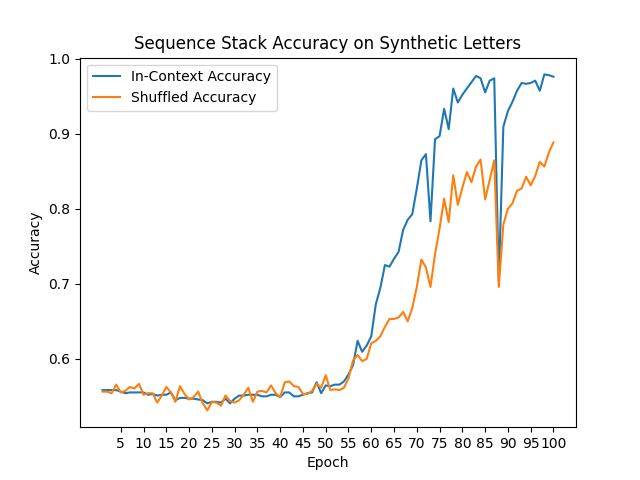
\includegraphics[width=\textwidth]{figures/sequence_stack_mnist_like.png}
        \caption{}
        \label{resultsa}
    \end{subfigure}\begin{subfigure}{0.5\textwidth}
        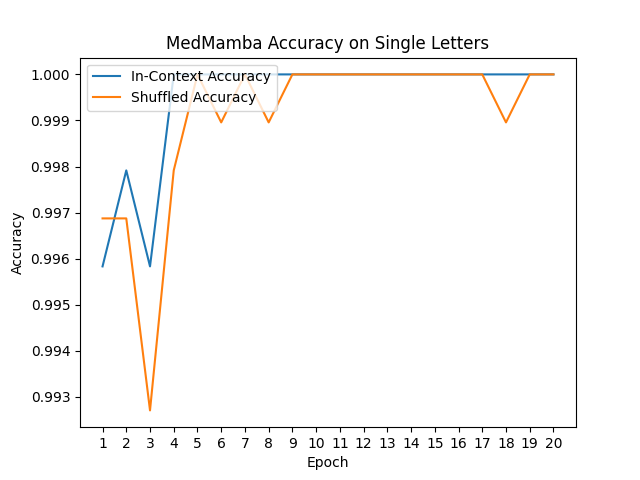
\includegraphics[width=\textwidth]{figures/medmamba_mnist_like.png}
        \caption{}
        \label{resultsb}
    \end{subfigure}
    \begin{subfigure}{0.5\textwidth}
        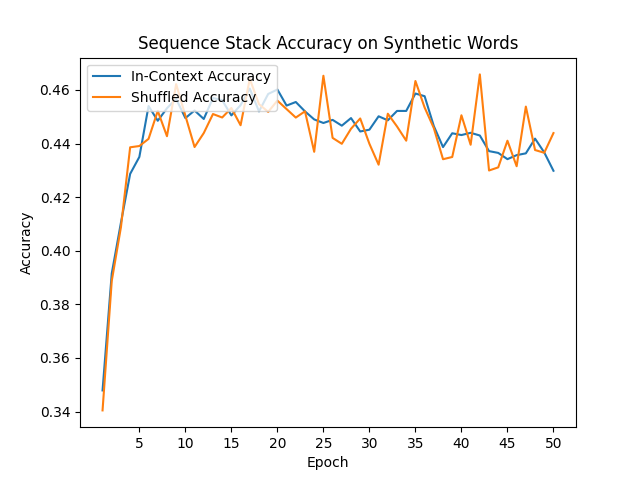
\includegraphics[width=\textwidth]{figures/sequence_stack_words.png}
        \caption{}
        \label{resultsc}
    \end{subfigure}\begin{subfigure}{0.5\textwidth}
        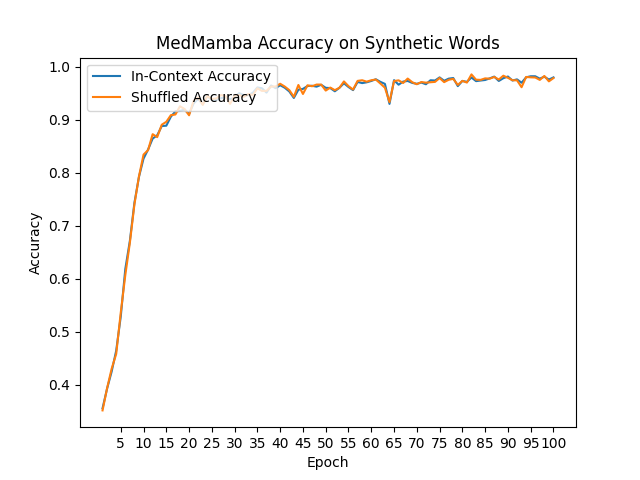
\includegraphics[width=\textwidth]{figures/medmamba_words.png}
        \caption{}
        \label{resultsd}
    \end{subfigure}
    \begin{subfigure}{0.5\textwidth}
        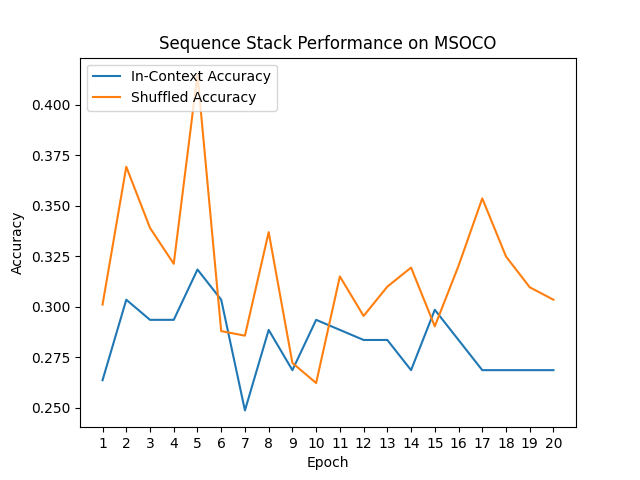
\includegraphics[width=\textwidth]{figures/sequence_stack_mscoco.png}
        \caption{}
        \label{resultse}
    \end{subfigure}\begin{subfigure}{0.5\textwidth}
        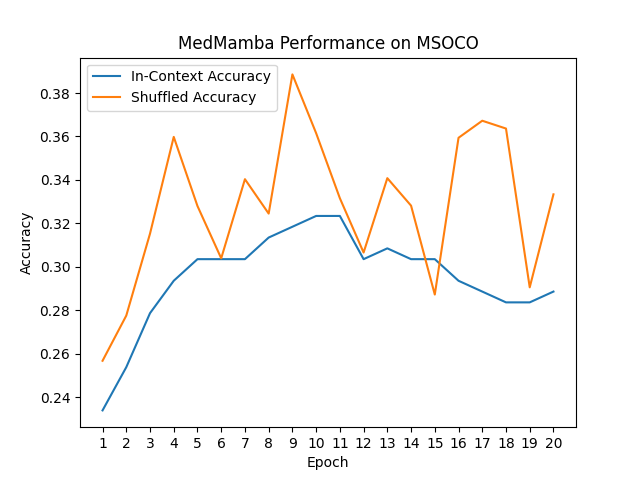
\includegraphics[width=\textwidth]{figures/medmamba_mscoco.png}
        \caption{}
        \label{resultsf}
    \end{subfigure}
    \caption{Graphs of results}
    \label{resultslide}
\end{figure}
As shown in Figure \ref{resultsa} and Figure \ref{resultsb}, both the sequence
stack model and the medmamba-based model perform better when validated on
in-context data as opposed to shuffled contexts.

However, as shown in Figure \ref{resultsc} and Figure \ref{resultsd}, the
in-context accuracy boost disappears.
In addition, we find that the overall performance degrades significantly.
For MedMamba, the accuracy dropped from 100\% down to around 98\%.
For sequence stack, the accuracy dropped from 100\% down to around 40\% for
in-context, and 80\% to 40\% for shuffled-contexts.

With the COCO-Text datasets, this trend worsens, likely due to the small dataset
size.
In particular, MedMamba now fails to achieve high accuracy in either validation
set.

One possible explanation is that the multi-character task requires Mamba to
store far more information in its internal state.
With single letters, the model can theoretically do the task by just remembering
the image data for the previous character.
However, with entire words, the model might have to memorize over 10 times the
amount of data.
In addition, the amount of data that the model is required to memorize varies
from word-to-word.

Previous work \cite{mambangram} has found the Mamba models generalize well when
tasked with copying fixed-length subsequences over varying distances, but they
fail to generalize when the length of the subsequence is varied.
An interpretation of these finding is that a Mamba and other SSMs are severely
limited by memory constraints.
In the single digit dataset, the model only strictly needs to memorize the the
image corresponding to a single digit.
However, with the word dataset, the model might have to memorize over ten times
the amount of information compared to in the single digit dataset.
This is since the model has to store all of it's letter labels until the end of
the word, when it can output its prediction and forget predictions.
This means that with the single digit case, the model can easily memorize the
current image with spare memory to store context info.
However, in the whole word dataset, the model might simply be training to
memorize larger and larger words, leaving no free memory for memorizing
context-specific details.

We also found that the MedMamda-based model does significantly better compared
to the sequence stack model.
This could be due to the inclusion of the CNN layers and down-sampling, which
could allow the model to more efficiently extract different features in the
image.

The same analysis applies to the results for COCO-Text.
